% Full instructions available at:
% https://github.com/elauksap/focus-beamertheme

\documentclass{beamer}
\usetheme{focus}

\usepackage[utf8]{inputenc}
\usepackage[T1]{fontenc}
\usepackage[french]{babel}

% \usepackage{subcaption}

\usepackage{graphics}
\usepackage{graphicx}

\usepackage{pifont}% http://ctan.org/pkg/pifont
\newcommand{\cmark}{\color{example}\ding{51}}%
\newcommand{\xmark}{\color{red}\ding{55}}%
\newcommand{\fmark}{\ding{229}}%
\newcommand{\itemc}{\item[\cmark]}%
\newcommand{\itemx}{\item[\xmark]}%
\newcommand{\itemf}{\item[\fmark]}%

\usepackage{siunitx}

\title{Convertir l'énergie}
\subtitle{}
\author{ETT - Cours}
\titlegraphic{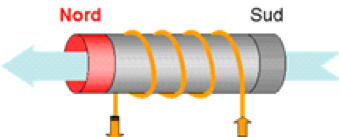
\includegraphics[width=.2\textwidth]{images/indu_aimant1}}
\institute{Lycée Louis Armand}
\date{25 novembre 2018}

\begin{document}
\begin{frame}{}

\end{frame}
    \begin{frame}
        \maketitle
    \end{frame}

    \begin{frame}
        \tableofcontents
    \end{frame}

    \section{Généralités}
    \begin{frame}{La fonction convertir}
      \centering
      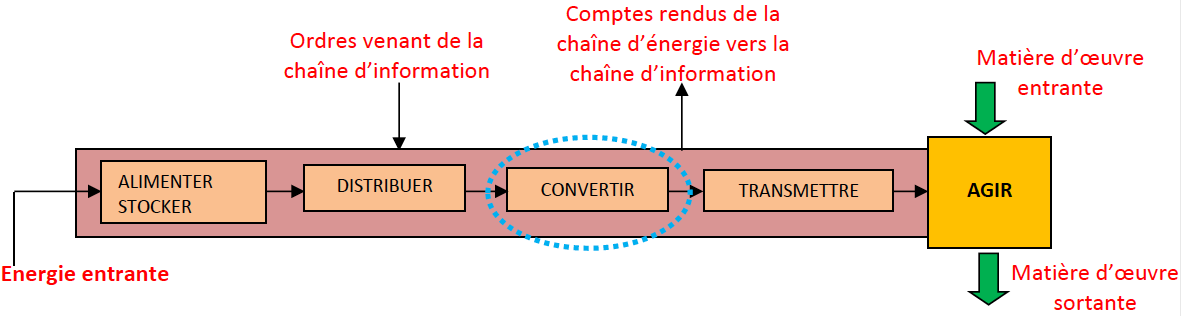
\includegraphics[width=\textwidth]{images/S03_C03}
    \end{frame}

    % \begin{frame}{}
    %   \centering
    %   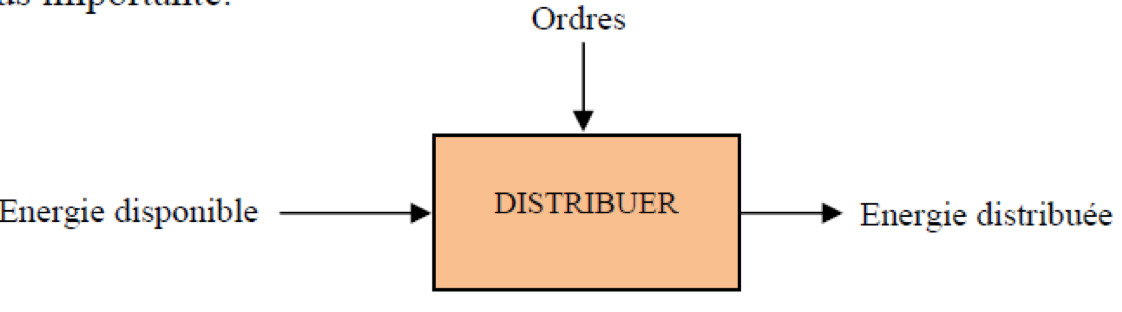
\includegraphics[width=.6\textwidth]{images/distribuer}
    % \end{frame}

    \begin{frame}{Définition}
      \begin{alertblock}{Le bloc Convertir}
        La fonction « Convertir » de la chaîne d'énergie convertit l'énergie fournie au système en énergie \textbf{utile}.
      \end{alertblock}

      \visible<2->{\begin{exampleblock}{Propriétés}
        Les composants réalisant la conversion d’énergie sont appelés « actionneurs » : ils permettent de convertir l'énergie reçue en travail utile.
      \end{exampleblock}}
    \end{frame}

    \begin{frame}{Quelques exemples}
      \centering
      \begin{figure}[h]
        \centering
          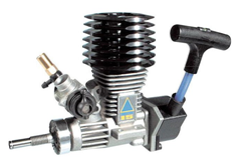
\includegraphics[width=0.24\textwidth]{images/moteur_thermique}
          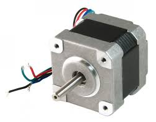
\includegraphics[width=0.24\textwidth]{images/moteur_paspas}
          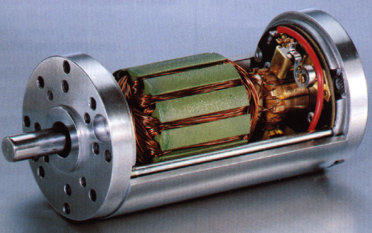
\includegraphics[width=0.24\textwidth]{images/moteur_continu}
          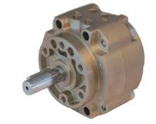
\includegraphics[width=0.24\textwidth]{images/verin_rotatif}\\

          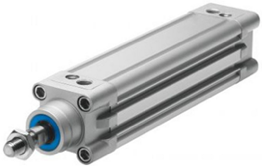
\includegraphics[width=0.24\textwidth]{images/verin_pneu}
          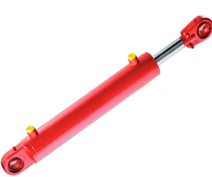
\includegraphics[width=0.24\textwidth]{images/verin_hydrqu}
          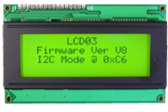
\includegraphics[width=0.24\textwidth]{images/afficheur}
          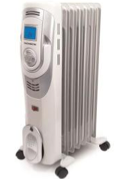
\includegraphics[width=0.24\textwidth]{images/radiateur}
        \caption{Quelques exemples d'actionneurs}
        \label{fig:exemples}
      \end{figure}
    \end{frame}

\section{Effet joule}
\begin{frame}{Fonctionnement d'un chauffage simple}
  \centering
  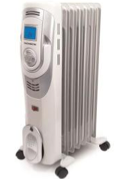
\includegraphics[width=0.1\textwidth]{images/radiateur}
  \begin{block}{Production de chaleur par effet joule}
    Lorsque les électrons se déplacent dans un conducteur, interagissent avec les atomes constitutifs de la matière. Cette interaction résiste à leur déplacement et crée de la chaleur.
  \end{block}

  \begin{alertblock}{A retenir}
    La puissance thermique dissipée par effet joule dans une résistance est égale à la puissance électrique qui traverse cette résistance.
    $$P=U\times I = R\times I^2$$.

    Cette puissance ne dépend que du courant.
  \end{alertblock}
\end{frame}

\section{Les vérins}

\begin{frame}{Fonctionnement d'un vérin}
  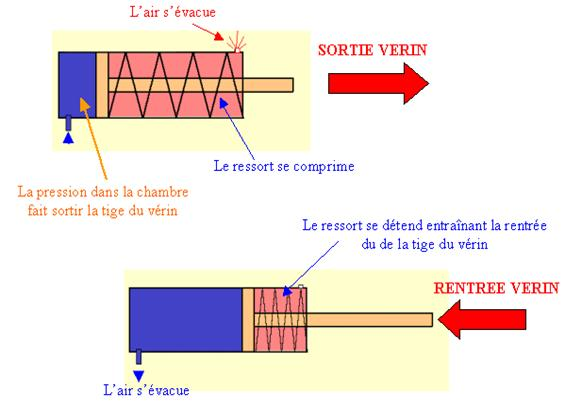
\includegraphics[width=.5\textwidth]{images/verin}
\end{frame}

\begin{frame}{Vérin simple et double effet}
  \begin{block}{Vérin simple effet}
    Les vérins « simple effet » n'ont qu'\textbf{une direction de travail}. Cela signifie qu'ils ne forcent que dans un sens. La tige du vérin est ramenée par un ressort.
  \end{block}
  \visible<2->{
  \begin{block}{Vérin double effet}
    Les vérins « double effet » ont \textbf{deux directions de travail}. Cela signifie qu'ils peuvent forcer dans les deux sens. Le fluide sous pression peut arriver d'un côté ou de l'autre du vérin pour faire rentrer ou sortir la tige selon l'effet désiré.
  \end{block}
  }
\end{frame}

\section{Les moteurs}

\begin{frame}{Généralités}
  \begin{alertblock}{Rotor et stator}
    Les moteurs électriques sont tous constitués d'un \textbf{stator} fixe par rapport auquel un \textbf{rotor} tourne.
  \end{alertblock}

  \centering
  \visible<2->{
  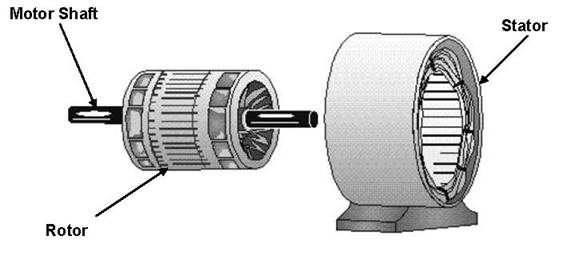
\includegraphics[width=.5\textwidth]{images/stator-Rotor}
  }
\end{frame}

\begin{frame}{Fonctionnement d'un moteur thermique}

\end{frame}


\begin{frame}{Champs magnétique à partir d'une bobine}
  \centering
  \only<1>{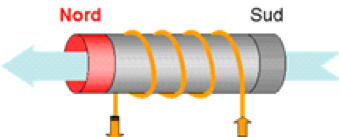
\includegraphics[width=0.5\textwidth]{images/indu_aimant1}}
  \only<2>{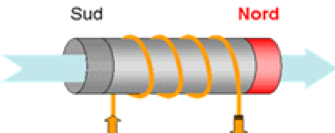
\includegraphics[width=0.5\textwidth]{images/indu_aimant2}}
\end{frame}

\begin{frame}{Moteur synchrone}
  \centering
  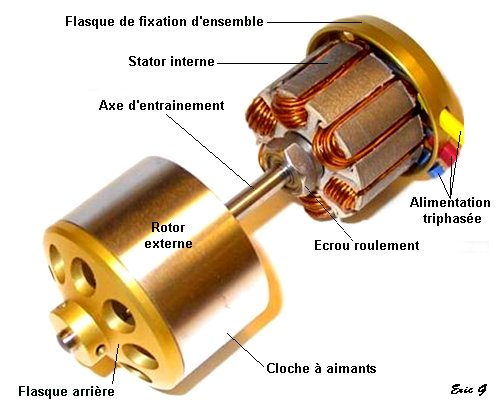
\includegraphics[width=.5\textwidth]{images/moteur11}
\end{frame}

\begin{frame}{Moteur à courant continu}
  \centering
  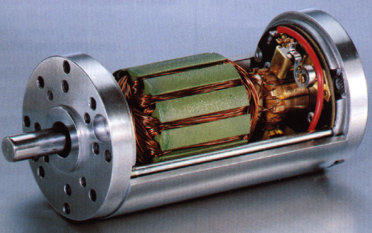
\includegraphics[width=.5\textwidth]{images/moteur_continu}\\
  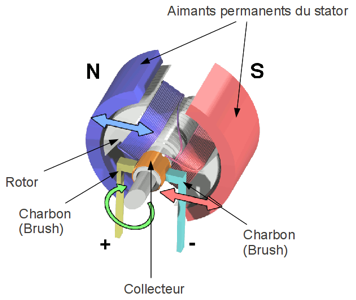
\includegraphics[width=.5\textwidth]{images/moteur_continu_explose}
\end{frame}

\begin{frame}{Moteur à courant continu}
  \begin{alertblock}{A retenir}
    Le couple d'un moteur à courant continu varie en fonction de son courant d'alimentation
  \end{alertblock}

  \begin{alertblock}{A retenir}
    La vitesse d'un moteur à courant continu varie en fonction de sa tension d'alimentation
  \end{alertblock}
\end{frame}

    \begin{frame}[focus]
        Questions ?
    \end{frame}

    \appendix
\end{document}
